\section{Discussion and Conclusion}
\label{sec:discussion}
\label{sec:conclusion}

\looseness=-1
Formal verification's value depends on the \emph{independence} of its inputs, not the soundness of its logic. SICA reduces to majority vote under source-attribution scoring (Observation~1), and 27 training-free variants fail to escape; symbolic confirmation bias holds across nine models (7B to frontier). Three lightweight diagnostics predict failure from a $K{=}12$ pilot (\S\ref{sec:diagnostic-framework}).

\looseness=-1
For the broader neuro-symbolic community, our results expose a structural limitation of self-extraction pipelines: when the same model generates both reasoning and formal constraints, the symbolic layer inherits the model's distributional prior rather than providing an independent check. This limitation is not specific to logical constraint extraction; it applies to any self-verification paradigm where the verifier shares the generator's knowledge boundary \citep{huang2024selfcorrect}.

\begin{figure}[t]
\centering
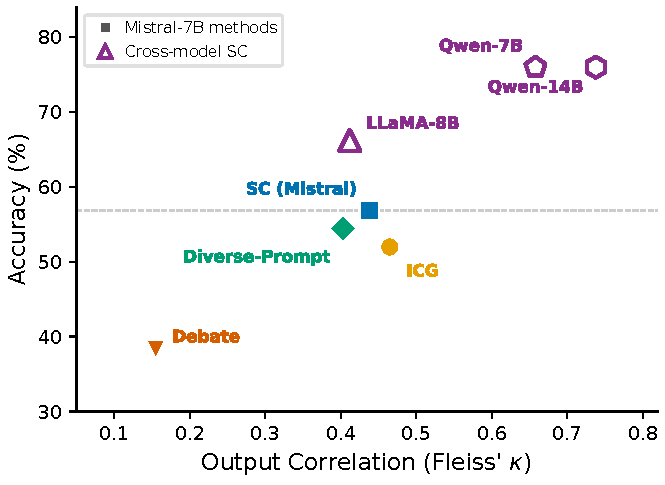
\includegraphics[width=\columnwidth]{figures/f6_kappa_accuracy_scatter}
\caption{Independence--accuracy trade-off across 27 remediation strategies on FOLIO ($n = 204$). Dashed line: Mistral-7B SC baseline.}
\label{fig:kappa-accuracy}
\end{figure}

\looseness=-1
We formalize the link between these findings via the \emph{Conditional Correction Ratio}: $\text{CCR}(V, G) = \log \frac{P(V \text{ correct} \mid G \text{ wrong})}{P(V \text{ correct} \mid G \text{ correct})}$. All same-model SICA conditions yield $\text{CCR} < 0$ (shared bias), while cross-architecture NLI pairs achieve $\text{CCR} > 0$ (preferential error correction); CCR correlates with combo gain ($\rho = 0.84$, $p = 0.014$; Appendix~\ref{app:cil}).

\looseness=-1
Cross-architecture verification escapes only when the verifier exceeds generator accuracy (\S\ref{sec:cross-arch}); this points to \emph{architectural diversity} over scale as the key design principle. Trained verifiers (PRM \citep{lightman2024prm,wang2024mathshepherd}, ORM \citep{cobbe2021gsm8k}) succeed precisely because they break the $M{\to}T{\to}(A,C)$ generation structure with independently supervised signal; our NLI escape instantiates this principle without task-specific training ($+6.67$\,pp). For test-time compute scaling \citep{snell2025scaling}, our findings imply that allocating additional inference budget to self-consistent sampling yields diminishing returns once $K_\text{eff}$ saturates; redirecting compute toward structurally independent verification offers a more efficient path. Lightweight trained verification is a natural next step (Appendix~\ref{app:extended-discussion}).
